\documentclass{standalone}
\usepackage{tikz}
\usetikzlibrary{patterns, positioning}


\begin{document}
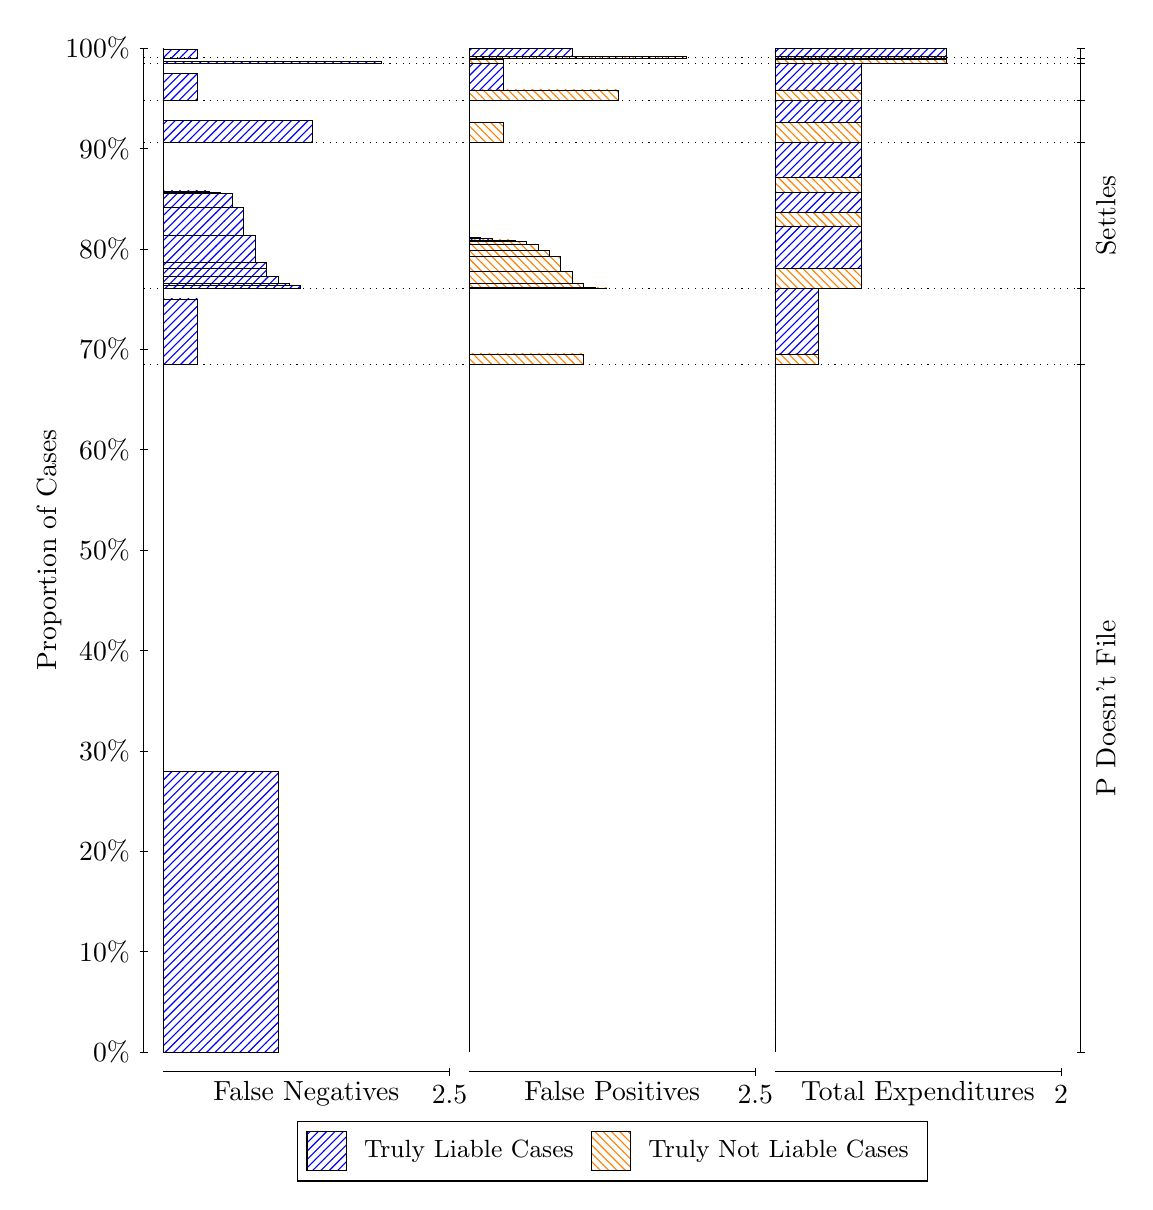
\begin{tikzpicture}
\draw[black, very thin] (1.5,1.75) -- (1.5,14.5);
\node[rotate=90, text=black, anchor=center] at (0.3, 8.125) {Proportion of Cases};
\draw[black, very thin] (1.45,1.75) -- (1.55,1.75);
\node[text=black, anchor=east] at (1.45, 1.75) {0\%};
\draw[black, very thin] (1.45,3.025) -- (1.55,3.025);
\node[text=black, anchor=east] at (1.45, 3.025) {10\%};
\draw[black, very thin] (1.45,4.3) -- (1.55,4.3);
\node[text=black, anchor=east] at (1.45, 4.3) {20\%};
\draw[black, very thin] (1.45,5.575) -- (1.55,5.575);
\node[text=black, anchor=east] at (1.45, 5.575) {30\%};
\draw[black, very thin] (1.45,6.85) -- (1.55,6.85);
\node[text=black, anchor=east] at (1.45, 6.85) {40\%};
\draw[black, very thin] (1.45,8.125) -- (1.55,8.125);
\node[text=black, anchor=east] at (1.45, 8.125) {50\%};
\draw[black, very thin] (1.45,9.4) -- (1.55,9.4);
\node[text=black, anchor=east] at (1.45, 9.4) {60\%};
\draw[black, very thin] (1.45,10.675) -- (1.55,10.675);
\node[text=black, anchor=east] at (1.45, 10.675) {70\%};
\draw[black, very thin] (1.45,11.95) -- (1.55,11.95);
\node[text=black, anchor=east] at (1.45, 11.95) {80\%};
\draw[black, very thin] (1.45,13.225) -- (1.55,13.225);
\node[text=black, anchor=east] at (1.45, 13.225) {90\%};
\draw[black, very thin] (1.45,14.5) -- (1.55,14.5);
\node[text=black, anchor=east] at (1.45, 14.5) {100\%};

\draw[black, very thin] (13.4,1.75) -- (13.4,14.5);
\draw[black, very thin] (13.35,1.75) -- (13.45,1.75);
\node[anchor=west] at (13.35, 1.75) {};
\draw[black, very thin] (13.35,10.482) -- (13.45,10.482);
\node[anchor=west] at (13.35, 10.482) {};
\draw[black, very thin] (13.35,11.448) -- (13.45,11.448);
\node[anchor=west] at (13.35, 11.448) {};
\draw[black, very thin] (13.35,13.3) -- (13.45,13.3);
\node[anchor=west] at (13.35, 13.3) {};
\draw[black, very thin] (13.35,13.835) -- (13.45,13.835);
\node[anchor=west] at (13.35, 13.835) {};
\draw[black, very thin] (13.35,14.307) -- (13.45,14.307);
\node[anchor=west] at (13.35, 14.307) {};
\draw[black, very thin] (13.35,14.376) -- (13.45,14.376);
\node[anchor=west] at (13.35, 14.376) {};
\draw[black, very thin] (13.35,14.5) -- (13.45,14.5);
\node[anchor=west] at (13.35, 14.5) {};

\draw[black, very thin, pattern color=blue, pattern=north east lines] (1.75,1.75) rectangle (3.2033,5.3133);
\draw[black, very thin, pattern color=orange, pattern=north west lines] (1.75,5.3133) rectangle (1.75,10.482);
\draw[black, very thin, pattern color=blue, pattern=north east lines] (1.75,10.482) rectangle (2.186,11.313);
\draw[black, very thin, pattern color=orange, pattern=north west lines] (1.75,11.313) rectangle (1.75,11.448);
\draw[black, very thin, pattern color=blue, pattern=north east lines] (1.75,11.448) rectangle (3.494,11.481);
\draw[black, very thin, pattern color=blue, pattern=north east lines] (1.75,11.481) rectangle (3.3487,11.508);
\draw[black, very thin, pattern color=blue, pattern=north east lines] (1.75,11.508) rectangle (3.2033,11.604);
\draw[black, very thin, pattern color=blue, pattern=north east lines] (1.75,11.604) rectangle (3.058,11.705);
\draw[black, very thin, pattern color=blue, pattern=north east lines] (1.75,11.705) rectangle (3.058,11.775);
\draw[black, very thin, pattern color=blue, pattern=north east lines] (1.75,11.775) rectangle (2.9127,12.124);
\draw[black, very thin, pattern color=blue, pattern=north east lines] (1.75,12.124) rectangle (2.7673,12.475);
\draw[black, very thin, pattern color=blue, pattern=north east lines] (1.75,12.475) rectangle (2.622,12.65);
\draw[black, very thin, pattern color=blue, pattern=north east lines] (1.75,12.65) rectangle (2.4767,12.667);
\draw[black, very thin, pattern color=blue, pattern=north east lines] (1.75,12.667) rectangle (2.3313,12.686);
\draw[black, very thin, pattern color=orange, pattern=north west lines] (1.75,12.686) rectangle (1.75,13.3);
\draw[black, very thin, pattern color=blue, pattern=north east lines] (1.75,13.3) rectangle (3.6393,13.581);
\draw[black, very thin, pattern color=orange, pattern=north west lines] (1.75,13.581) rectangle (1.75,13.835);
\draw[black, very thin, pattern color=blue, pattern=north east lines] (1.75,13.835) rectangle (2.186,14.173);
\draw[black, very thin, pattern color=orange, pattern=north west lines] (1.75,14.173) rectangle (1.75,14.307);
\draw[black, very thin, pattern color=blue, pattern=north east lines] (1.75,14.307) rectangle (4.5113,14.326);
\draw[black, very thin, pattern color=orange, pattern=north west lines] (1.75,14.326) rectangle (1.75,14.376);
\draw[black, very thin, pattern color=blue, pattern=north east lines] (1.75,14.376) rectangle (2.186,14.481);
\draw[black, very thin, pattern color=orange, pattern=north west lines] (1.75,14.481) rectangle (1.75,14.5);
\draw[black, very thin, pattern color=orange, pattern=north west lines] (5.6333,1.75) rectangle (5.6333,6.9188);
\draw[black, very thin, pattern color=blue, pattern=north east lines] (5.6333,6.9188) rectangle (5.6333,10.482);
\draw[black, very thin, pattern color=orange, pattern=north west lines] (5.6333,10.482) rectangle (7.0867,10.617);
\draw[black, very thin, pattern color=blue, pattern=north east lines] (5.6333,10.617) rectangle (5.6333,11.448);
\draw[black, very thin, pattern color=orange, pattern=north west lines] (5.6333,11.448) rectangle (7.3773,11.453);
\draw[black, very thin, pattern color=orange, pattern=north west lines] (5.6333,11.453) rectangle (7.232,11.457);
\draw[black, very thin, pattern color=orange, pattern=north west lines] (5.6333,11.457) rectangle (7.0867,11.515);
\draw[black, very thin, pattern color=orange, pattern=north west lines] (5.6333,11.515) rectangle (6.9413,11.662);
\draw[black, very thin, pattern color=orange, pattern=north west lines] (5.6333,11.662) rectangle (6.796,11.85);
\draw[black, very thin, pattern color=orange, pattern=north west lines] (5.6333,11.85) rectangle (6.6507,11.933);
\draw[black, very thin, pattern color=orange, pattern=north west lines] (5.6333,11.933) rectangle (6.5053,12.007);
\draw[black, very thin, pattern color=orange, pattern=north west lines] (5.6333,12.007) rectangle (6.36,12.04);
\draw[black, very thin, pattern color=orange, pattern=north west lines] (5.6333,12.04) rectangle (6.2147,12.062);
\draw[black, very thin, pattern color=blue, pattern=north east lines] (5.6333,12.062) rectangle (5.924,12.081);
\draw[black, very thin, pattern color=blue, pattern=north east lines] (5.6333,12.081) rectangle (5.7787,12.098);
\draw[black, very thin, pattern color=blue, pattern=north east lines] (5.6333,12.098) rectangle (5.6333,13.3);
\draw[black, very thin, pattern color=orange, pattern=north west lines] (5.6333,13.3) rectangle (6.0693,13.554);
\draw[black, very thin, pattern color=blue, pattern=north east lines] (5.6333,13.554) rectangle (5.6333,13.835);
\draw[black, very thin, pattern color=orange, pattern=north west lines] (5.6333,13.835) rectangle (7.5227,13.969);
\draw[black, very thin, pattern color=blue, pattern=north east lines] (5.6333,13.969) rectangle (6.0693,14.307);
\draw[black, very thin, pattern color=orange, pattern=north west lines] (5.6333,14.307) rectangle (6.0693,14.357);
\draw[black, very thin, pattern color=blue, pattern=north east lines] (5.6333,14.357) rectangle (5.6333,14.376);
\draw[black, very thin, pattern color=orange, pattern=north west lines] (5.6333,14.376) rectangle (8.3947,14.395);
\draw[black, very thin, pattern color=blue, pattern=north east lines] (5.6333,14.395) rectangle (6.9413,14.5);
\draw[black, very thin, pattern color=orange, pattern=north west lines] (9.5167,1.75) rectangle (9.5167,6.9188);
\draw[black, very thin, pattern color=blue, pattern=north east lines] (9.5167,6.9188) rectangle (9.5167,10.482);
\draw[black, very thin, pattern color=orange, pattern=north west lines] (9.5167,10.482) rectangle (10.062,10.617);
\draw[black, very thin, pattern color=blue, pattern=north east lines] (9.5167,10.617) rectangle (10.062,11.448);
\draw[black, very thin, pattern color=orange, pattern=north west lines] (9.5167,11.448) rectangle (10.607,11.699);
\draw[black, very thin, pattern color=blue, pattern=north east lines] (9.5167,11.699) rectangle (10.607,12.24);
\draw[black, very thin, pattern color=orange, pattern=north west lines] (9.5167,12.24) rectangle (10.607,12.41);
\draw[black, very thin, pattern color=blue, pattern=north east lines] (9.5167,12.41) rectangle (10.607,12.667);
\draw[black, very thin, pattern color=orange, pattern=north west lines] (9.5167,12.667) rectangle (10.607,12.859);
\draw[black, very thin, pattern color=blue, pattern=north east lines] (9.5167,12.859) rectangle (10.607,13.3);
\draw[black, very thin, pattern color=orange, pattern=north west lines] (9.5167,13.3) rectangle (10.607,13.554);
\draw[black, very thin, pattern color=blue, pattern=north east lines] (9.5167,13.554) rectangle (10.607,13.835);
\draw[black, very thin, pattern color=orange, pattern=north west lines] (9.5167,13.835) rectangle (10.607,13.969);
\draw[black, very thin, pattern color=blue, pattern=north east lines] (9.5167,13.969) rectangle (10.607,14.307);
\draw[black, very thin, pattern color=orange, pattern=north west lines] (9.5167,14.307) rectangle (11.697,14.357);
\draw[black, very thin, pattern color=blue, pattern=north east lines] (9.5167,14.357) rectangle (11.697,14.376);
\draw[black, very thin, pattern color=orange, pattern=north west lines] (9.5167,14.376) rectangle (11.697,14.395);
\draw[black, very thin, pattern color=blue, pattern=north east lines] (9.5167,14.395) rectangle (11.697,14.5);
\draw[black, dotted] (1.5,10.482) -- (13.4,10.482);
\draw[black, dotted] (1.5,11.448) -- (13.4,11.448);
\draw[black, dotted] (1.5,13.3) -- (13.4,13.3);
\draw[black, dotted] (1.5,13.835) -- (13.4,13.835);
\draw[black, dotted] (1.5,14.307) -- (13.4,14.307);
\draw[black, dotted] (1.5,14.376) -- (13.4,14.376);
\draw[black, very thin] (1.75,1.5) -- (5.3833,1.5);
\node[text=black, anchor=north] at (3.5667, 1.5) {False Negatives};
\draw[black, very thin] (5.3833,1.45) -- (5.3833,1.55);
\node[text=black, anchor=north] at (5.3833, 1.45) {2.5};

\draw[black, very thin] (5.6333,1.5) -- (9.2667,1.5);
\node[text=black, anchor=north] at (7.45, 1.5) {False Positives};
\draw[black, very thin] (9.2667,1.45) -- (9.2667,1.55);
\node[text=black, anchor=north] at (9.2667, 1.45) {2.5};

\draw[black, very thin] (9.5167,1.5) -- (13.15,1.5);
\node[text=black, anchor=north] at (11.333, 1.5) {Total Expenditures};
\draw[black, very thin] (13.15,1.45) -- (13.15,1.55);
\node[text=black, anchor=north] at (13.15, 1.45) {2};

\node[text=black, centered, rotate=90] at (13.72, 6.116) {P Doesn't File};

\node[text=black, centered, rotate=90] at (13.72, 12.374) {Settles};





\draw (7.449999999999999,1.5) node[draw=none] (baseCoordinate) {};
\begin{scope}[align=center]
        \matrix[scale=0.5, draw=black, below=0.5cm of baseCoordinate, nodes={draw}, column sep=0.1cm]{
            \node[rectangle, draw, minimum width=0.5cm, minimum height=0.5cm, pattern color=blue, pattern=north east lines] {}; &
            \node[draw=none, font=\small, text=black] (B) {Truly Liable Cases}; &
            \node[rectangle, draw, minimum width=0.5cm, minimum height=0.5cm, pattern color=orange, pattern=north west lines] {}; &
            \node[draw=none, font=\small, text=black] (B) {Truly Not Liable Cases}; \\
            };
\end{scope}

\end{tikzpicture}
\end{document}